\documentclass[11pt, oneside]{article}   	% use "amsart" instead of "article" for AMSLaTeX format
\usepackage{geometry}                		% See geometry.pdf to learn the layout options. There are lots.
\geometry{letterpaper}                   		% ... or a4paper or a5paper or ... 
%\geometry{landscape}                		% Activate for rotated page geometry
\usepackage[parfill]{parskip}    		% Activate to begin paragraphs with an empty line rather than an 
\usepackage{graphicx}				% Use pdf, png, jpg, or eps§ with pdflatex; use eps in DVI 
\usepackage{amssymb}
\usepackage{booktabs}
\usepackage{listings}
\usepackage{color}
\usepackage{makecell}
\usepackage{multirow}
\usepackage{changepage}
\usepackage{soul}
\usepackage{textcomp}
\usepackage{courier}

\lstset{ % General setup for the package
	basicstyle = \ttfamily\scriptsize,
	numberstyle=\tiny,
	numbers=none,
	frame=tb,
	tabsize=4,
	columns=fixed,
	showstringspaces=false,
	showtabs=false,
	keepspaces,
	commentstyle=\color{red},
	keywordstyle=\color{blue},
	backgroundcolor=\color[gray]{0.95}
}

\lstdefinelanguage{Rplus}{%
  language     = R,
  alsoletter   = {.},
  morekeywords = {[2] TRUE, FALSE},
  morestring   = [s]'',
  morestring   = [s]"",
  keywordstyle = \color[RGB]{0,0,0},
  keywordstyle = [2]\color[RGB]{0,0,194},
  commentstyle = \color[RGB]{22,89,52},
  stringstyle  = \color[RGB]{22,89,52},
  literate=%
    {0}{{{\color[RGB]{0,0,194}0}}}1
    {1}{{{\color[RGB]{0,0,194}1}}}1
    {2}{{{\color[RGB]{0,0,194}2}}}1
    {3}{{{\color[RGB]{0,0,194}3}}}1
    {4}{{{\color[RGB]{0,0,194}4}}}1
    {5}{{{\color[RGB]{0,0,194}5}}}1
    {6}{{{\color[RGB]{0,0,194}6}}}1
    {7}{{{\color[RGB]{0,0,194}7}}}1
    {8}{{{\color[RGB]{0,0,194}8}}}1
    {9}{{{\color[RGB]{0,0,194}9}}}1
}

\lstdefinelanguage{SPSS}
{
  sensitive    = false,
  alsoletter   = {/},
  morekeywords = {[1] data, begin, end, value, labels, manova, unianova, oneway, anova                   , compute, execute, list, variable, graph},
  morekeywords = {[2] ALL, AND, BY, EQ, GE, GT, LE, LT, NE, NOT, OR, TO, WITH,                          BOXPLOTS, unique, hierarchical, experimental, free, tukey, sstype,                    opower, test},
  morekeywords = {[3] /omeans, /design, /method, /posthoc, /print, /ranges, /contrast,                   /plot, /errorbar, /statistics},
  morekeywords = {[4] lmatrix, sterror},
  morecomment  = [s]*.,
  morecomment  = [s]{/*}{*/},
  }

\lstdefinestyle{SPSSstyle}
{
  language     = SPSS,
  upquote      = true,
  keywordstyle = {[1] \color[RGB]{0,0,114}\bfseries},
  keywordstyle = {[2] \color[RGB]{130,37,0}},
  keywordstyle = {[3] \color[RGB]{29,112,0}},
  keywordstyle = {[4] \color[RGB]{248,143,35}},
  commentstyle = \color[RGB]{109,109,109},
  breaklines   = true,
  columns      = fullflexible,
  rulecolor    = \color{black},  
}

\newenvironment{answer}{\begin{adjustwidth}{.6cm}{}\bfseries}{\end{adjustwidth}}

\title{Problem Set 2: Answer Key}
\author{PSYCH 613}
%\setlength{\parindent}{0.25in}
\date{}							% Activate to display a given date or no date

\begin{document}
\maketitle

1. Working with a source table.

(a) Complete the ANOVA source table given below. This problem is completed by hand with the help of a calculator or Excel; one can't use SPSS or R on this one. (2 points)

\begin{answer}
For the purposes of this Problem Set, we define the following variables as:

\indent{N = Total number of subjects}

\indent{T = Total number of between-subjects groups}

Values are calculated using the following table. Bolded numbers were already entered.

\begin{table}[h!]
	\begin{center}
		\label{tab:table1}
 		 	\begin{tabular}{ccccc}
   			\toprule
   			Source & SS & df & MS & F\\
  			 \midrule
   			between & \makecell{$SST = SSB + SSW \Rightarrow$ \\ $SSB = SST - SSW$} & \textbf{4} & $MSB = SSB / df_b$ & $F = MSB / MSW$\\
   			within & \textbf{420} & \makecell{$df_t = df_b + df_w \Rightarrow$ \\$ df_w = df_t - df_b$} & $MSW = SSW / df_w$\\
   			total & \textbf{480} & \textbf{64}\\
			\bottomrule
		\end{tabular}
	\end{center}
\end{table}

Then, filling in the variables from the table: 

\begin{table}[h!]
	\begin{center}
		\label{tab:table2}
 		 	\begin{tabular}{ccccc}
   			\toprule
   			Source & SS & df & MS & F\\
  			 \midrule
   			between & \makecell{$SSB=SST-SSW$ \\ $= 480-420=60$} & \textbf{4} & \makecell{ $MSB=SSB/df_b$ \\ $=60/4=15$ } & \makecell{ $F=MSB / MSW$ \\ $=15/7=2.143$ } \\
   			within & \textbf{420} & \makecell{ $df_w=df_t-df_b$ \\ $ =64-4=60$ } & \makecell{ $MSW=SSW/df_w$ \\ $=420/60=7$}\\
   			total & \textbf{480} & \textbf{64}\\
			\bottomrule
		\end{tabular}
	\end{center}
\end{table}

\end{answer}

(b) How many levels did the independent variable include? (2 points)

\begin{answer}
$df_b = T - 1 \Rightarrow T = df_b  + 1 = 4 + 1 = 5$
\end{answer}

(c) How many total subjects were in the study? (2 points)
\begin{answer}
$df_t = N - 1  \Rightarrow N = df_t  + 1 = 64 + 1 = 65$
\end{answer}
(d) What is the $F_{critical} $(using $\alpha = 0.05$) that you would use to test the observed $F$? (2 points)
\begin{answer}
We can calculate $F_{critical}$ with
\end{answer}
Excel
\begin{lstlisting}
= finv(.05, 4, 60)
\end{lstlisting}
R
\begin{lstlisting}[language=Rplus]
qf(.95, 4, 60)
\end{lstlisting}
\begin{answer}
$F_{critical} = 2.525$
\end{answer}
(e) Is the omnibus F (the observed F) statistically significant? Explain why or why not? (2 points)
\begin{answer}
The calculations show that $F(4,60)_{observed} = 2.143 < F(4,60)_{critical} = 2.525$. Since the observed $F$ value is smaller than the critical $F$ value, we fail to reject the null hypothesis. 
\end{answer}
(f)  What is the $R^2$ value corresponding to these data? State in words what $R^2$ means (even though you don't know the specifics of this study such as means, dependent variable, manipulation, etc.)? (2 points)

\begin{answer}

$R^2 = SSB / SST = 60 / 480 = 0.125$

This means that $12.5\%$ of the total variance is due to the differences between group means. This can be related to the pie plot, where the SSB variance is $12.5\%$ so the SSW variance must be $87.5\%$. 

\end{answer}

2. A statistics lecturer was investigating different teaching styles. She thought that the best way to teach the course was to have the following three components: conceptual discussion, examples illustrating computation, and exercises involving the computer. She conducts a study to test this hunch. One year she teaches the course only at a conceptual level (Group A). The second year she teaches at a conceptual level and adds examples illustrating computation (Group B). The third year she includes all three components: conceptual level, examples, and computer exercises (Group C). There are 8 students each year. All students took the identical final exam. The dependent measure is the total score on a standardized exam. [Data table removed].

(a) Enter data into SPSS or R and show your syntax. (2 points)

SPSS Syntax
\begin{lstlisting}[style=SPSSstyle]
DATA LIST FREE / group grade.
BEGIN DATA.
1 70
1 56
1 56
1 49
1 56
1 57
1 49
1 60
2 70
2 69
2 65
2 81
2 47
2 64
2 62
2 72
3 73
3 77
3 82
3 72
3 79
3 73
3 84
3 82
END DATA.

VARIABLE LABELS group 'Learning strategy'.
VALUE LABELS group 1 'Conceptual learning' 2 'Conceptual and examples' 
3 'Conceptual, examples, and computer exercises'.
\end{lstlisting}

R Syntax
\begin{lstlisting}[language=Rplus]
grade = c(70,56,56,49,56,57,49,60,70,69,65,81,47,64,62,72,73,77,82,72,79,73,84,82)
group = c(rep("A", 8),rep("B", 8),rep("C", 8))
data = data.frame(Group=group,Grade=grade)
levels(data$Group)<-c("Conceptual learning",
"Conceptual+Examples","Conceptual\n+Examples\n+Computer")
\end{lstlisting}

(b) From what you know about the design, write the structural model that the researcher is most likely testing. Label each term clearly and list the statistical assumptions that will be required to test this structural model. (2 points)
\begin{answer}
Structural model for one-way ANOVA

$Y_{ij} = \mu + \alpha_i + \epsilon_{ij}$

This means that our individual data points, individual $Y_{ij}$ points, are being estimated by a grand mean, $\mu$, plus a deviation from the mean for each group, $\alpha_i$, and some error for each item that you're fitting, $\epsilon_{ij}$. In this example, each $i$ corresponds to a group (conceptual level group, conceptual level with examples group, conceptual level with examples and computer exercises group), whereas each $j$ corresponds to an individual within each group. Each $\alpha_i$ corresponds to a group effect or treatment effect for each group under consideration (e.g., conceptual level only; conceptual level with examples; conceptual level, examples, and computer exercises).

Assumptions of one-way ANOVA

The assumptions for the one-way analysis of variance are the same as for the t-tests we performed in Lecture Notes $\#$1: Normally distributed data (i.e., roughly symmetric distribution on boxplot), equality of variances (no extreme discrepancy in length of IQR or whiskers on boxplot), and independence.
\end{answer}
(c) Compute estimates of $\mu$ and the three $\alpha$'s in the structural model (by hand, show your work). (2 points)
\begin{answer}
As in the lecture notes, $i$ denotes groups and $j$ denotes individuals within groups.

First, we need the group means $Y_i = \sum_{j=1}^{N}Y_j/N$ 

$Y_A=(70+56+56+49+56+57+49+60)/8 = 56.625$ 

$Y_B=(70+69+65+81+47+64+62+72)/8 = 66.25$

$Y_C=(73+77+82+72+79+73+84+82)/8 = 77.75 $

Grand mean = Mean of group means = $\mu=\sum_{i=1}^{T}Y_i/T$

$\mu = (56.625 + 66.25 + 77.75)/3 = 66.875$

NOTE: Since all groups have the same number of subjects, you can also calculate the grand mean as the mean of all subjects, $\mu=\sum_{i=1, j=1}^{i=T,j=N}Y_{ij}/N$. 

Deviations of group means from the grand mean $= \alpha_i=Y_i-\mu$ 

$\alpha_A=56.625-66.875=-10.25 $

$\alpha_B=66.25-66.875=-0.625 $

$\alpha_C=77.75-66.875=10.875 $

One thing that you may also notice is that sum of the $\alpha_i$ always sum to zero. You can relate this back to the graph in 2c by recognizing that the length of the lines representing your alpha values sum equally on the top and bottom of the mean. 
\end{answer}
(d) Provide a graph of the three means with ?1 standard error around each mean. (2 points)

SPSS Syntax
\begin{lstlisting}[style=SPSSstyle]
GRAPH 
/ERRORBAR (STERROR 1) grade BY group.
\end{lstlisting}

SPSS Output
\begin{figure}[h!]
  \centering
  \includegraphics[width=\linewidth]{2dplotSPSS.pdf}
  \caption{A graph of the three means with $\pm$ standard error around each mean.}
  \label{fig:SPSS1}
\end{figure}

R Syntax (There are many ways to plot error bars in R. This is one example.)
\begin{lstlisting}[language=Rplus]
#Plot groups means with +/- 1 SE
library(gplots)

#Calculate group standard errors
groupMeans = tapply(data$Grade,data$Group,mean)
groupSD = tapply(data$Grade,data$Group,sd)
groupN = tapply(data$Grade,data$Group,length)
groupSE = groupSD/sqrt(groupN)

plot.new()
plotCI(x = groupMeans, uiw = groupSE,liw = groupSE,err="y",xaxt="n",
ylab="Mean Test Scores (Error bars = +/- 1 se)",
main = "Mean Test Score by Teaching Method", xlab="Teaching Method")
labs=unique(data$Group)
axis(side=1, 1:3, labels=levels(data$Group))
\end{lstlisting}

R Output
\begin{figure}[h!]
  \centering
  \includegraphics[width=0.65\linewidth]{2dplotR.pdf}
  \caption{A graph of the three means with $\pm$ standard error around each mean.}
  \label{fig:R1}
\end{figure}

(e)Test the research hypothesis that there is a difference between the three means. Use $\alpha$ = 0.05. Interpret the result in words, you can refer to the graph in part 2d. (2 points)

SPSS Syntax
\begin{lstlisting}[style=SPSSstyle]
ONEWAY grade BY group  
/STATISTICS ALL.
\end{lstlisting}

SPSS Output
\begin{figure}[h!]
  \centering
  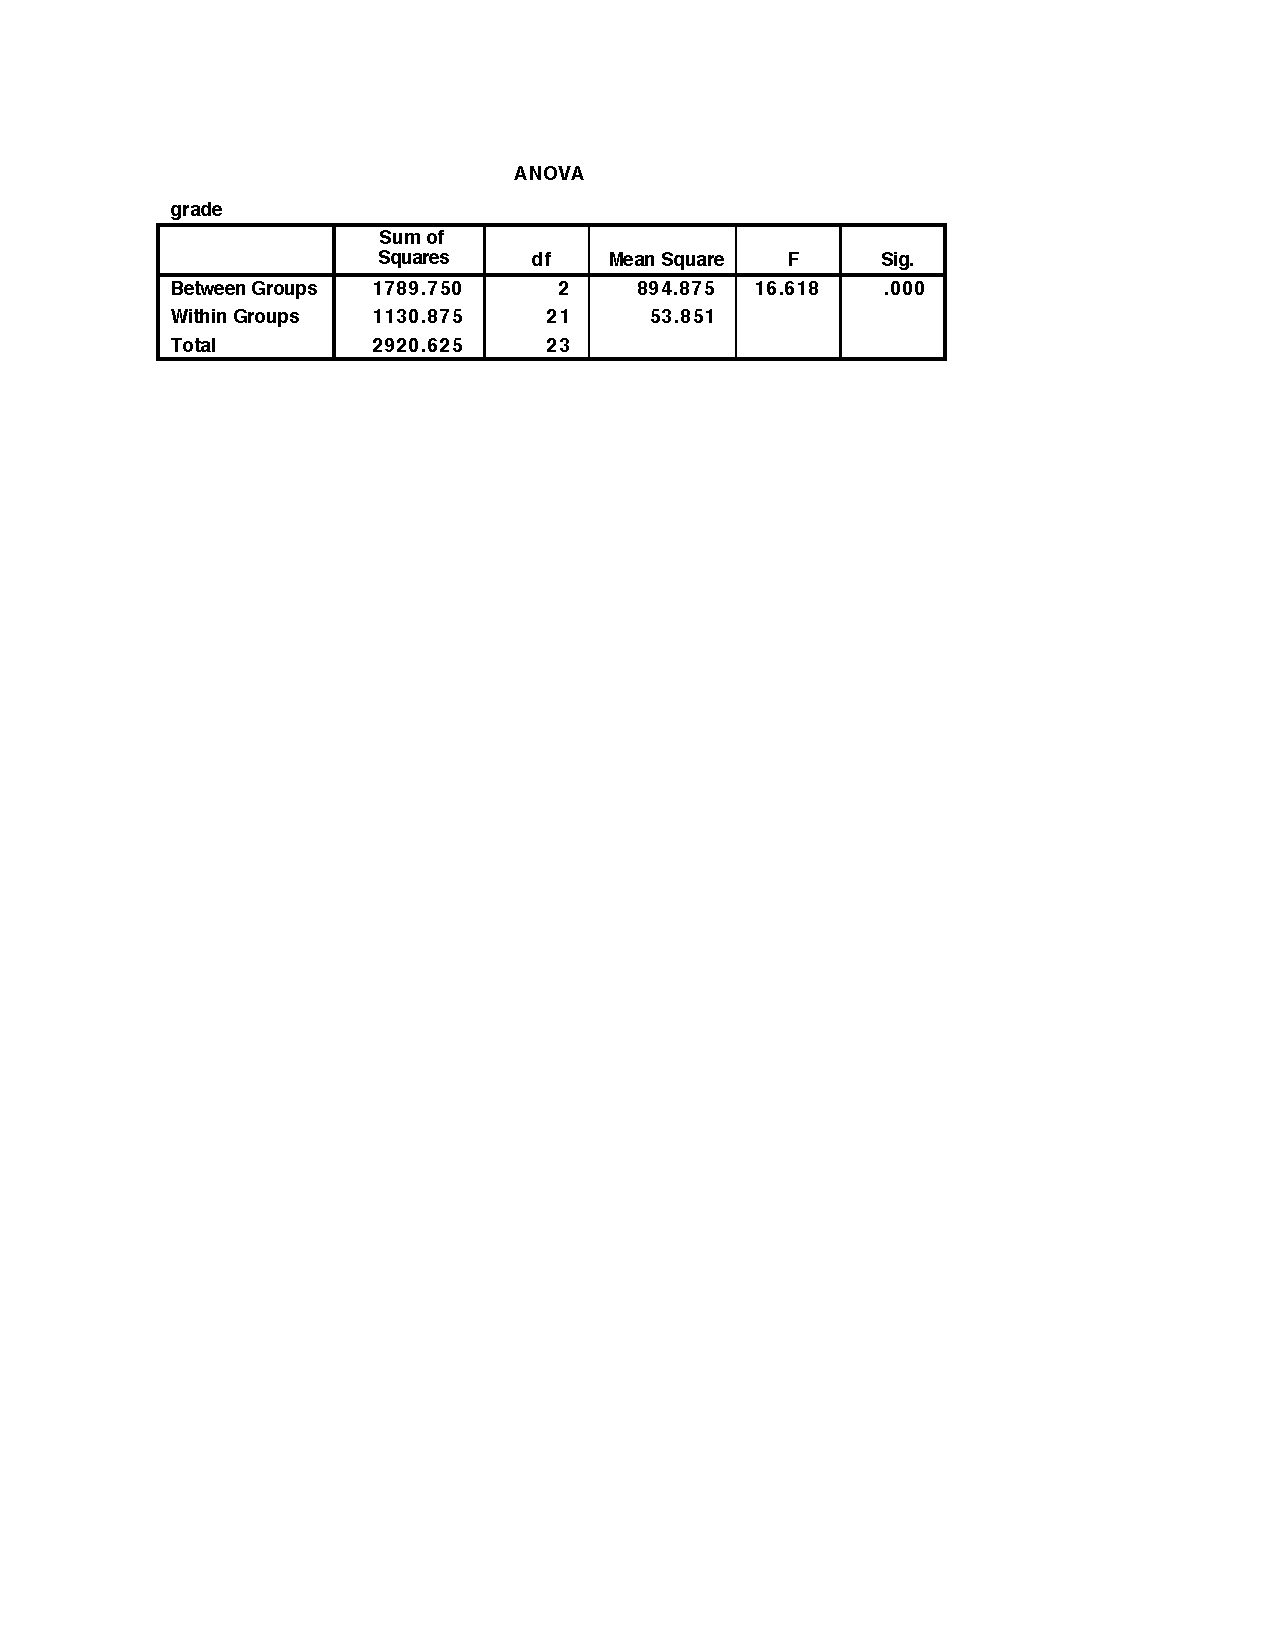
\includegraphics[width=\linewidth]{2eOutputSPSS.pdf}
  \caption{ANOVA Source Table.}
  \label{fig:SPSS2}
\end{figure}

R Syntax
\begin{lstlisting}[language=Rplus]
out <- aov(data$Grade ~ data$Group)
summary(out)
\end{lstlisting}

R Output
\begin{lstlisting}
            Df Sum Sq Mean Sq F value   Pr(>F)    
data$Group   2   1790   894.9   16.62 4.71e-05 ***
Residuals   21   1131    53.9                     
---
Signif. codes:  0 '***' 0.001 '**' 0.01 '*' 0.05 '.' 0.1 ' ' 1
\end{lstlisting}
\begin{answer}
I used a one-way analysis of variance and the null hypothesis that there was no difference between the final exam scores for Group A (conceptual level only), Group B (conceptual level and examples), and Group C (conceptual level, examples, and computer exercises) against the alternative hypothesis that there was a difference somewhere between the final exam scores for Group A, Group B, and Group C. I used the the qf(.95, 2, 21) command in R or =finv(.05, 2, 21) command in Excel to find $F_{critical} = 3.467$. Since $F_{observed}$ was larger than $F_{critical}$, we reject the null hypothesis and conclude that there is a a difference in test scores depending on the teaching method, $F_{obs}(2, 21) = 16.618$. 

I then used the graph in part 2d to see where the means likely differ. If the standard error bars overlap then the means should not differ, so the graph in part 2d suggests that Group C has higher test scores than both Group A and Group B, and that Group B has higher test scores than Group A.
\end{answer}


\end{document}  